\section{Establishing a deviation from the Standard Model}

In this section we describe a method for establishing a deviation from the Standard Model using the variables $\alpha_{T}$, $MH_{T}$ and $MH_{T}/H_{T}$.

First, we study the centrality of the leading jet of the standard model backgrounds and SUSY signals LM0 and LM1. Next, we investigate the contribution of each individual background to the total SM background. We define the variable $R_{\alpha T}$ which is the ratio of events which pass a cut on the value of $\alpha_{T}$ cut (the ``default'' value used is prompted by the all-hadronic analysis: N($\alpha_{T}>0.55$)) divided by the number of events below this cut (N($\alpha_{T}<0.55$)). We plot this ratio, $R_{\alpha T}$, as a function of the $|\eta|$ of the leading jet for the background only and the SUSY signal (LM0 and LM1) plus background cases. The analysis is repeated for the variables $MH_{T}$ and $MH_{T}/H_{T}$: a corresponding ratio of events passing a cut on the variable in question to those failing is plotted as a function of the $|\eta|$ of the leading jet.

\subsection{Centrality of the leading jet}

We decompose the Standard Model background into its components in order to study the $|\eta|$ of the leading jet for each background.  In figure \ref{fig:jeteta} the distributions of the SUSY signals (the LM0 and LM1 ``points'' are chosen as reference) are superimposed on the full SM background. Figure \ref{fig:jeteta}(a) shows the expected number of events in $100\textrm{pb}^{-1}$ after all selection cuts but $\alpha_{T}$.  The QCD background remains the largest contribution. QCD and W+jets events show, as expected, a flatish distribution in jet $\eta$, whereas the SUSY signal tends to be rather central. The Z+jets background contributes a small fraction of the total number of events and seems to be closer in shape to QCD.

A better comparison of the shapes of the different samples is provided by the corresponding, normalized to unit area, distributions plotted in figure \ref{fig:jeteta} right. The $b\bar{b}$ and QCD backgrounds are rather flat, compared to the other components. The $t\bar{t}$ background has a shape which is quite similar to that of the SUSY signals, especially in the low $\eta$ region.  The Z and W + jets events have approximately the same shape which is closer to that of the QCD events than the SUSY events.

\begin{figure}[h!]
\begin{minipage}[b]{0.5\linewidth}
\centering
{\label{fig:m$H_{T}$ov$H_{T}$}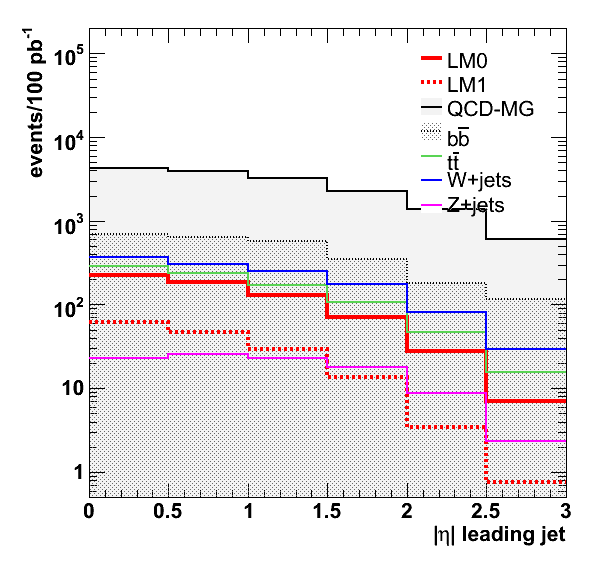
\includegraphics[scale=0.38]{./plots/JetEta.png}} 
\end{minipage}
\begin{minipage}[b]{0.5\linewidth}
\centering
{\label{fig:$H_{T}$}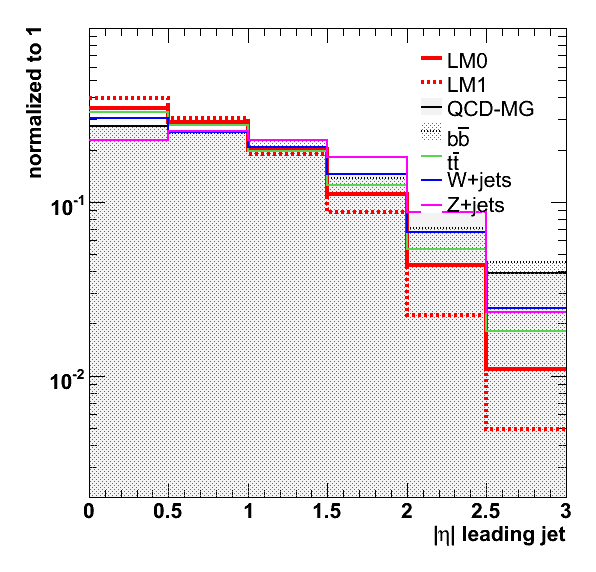
\includegraphics[scale=0.38]{./plots/JetEtaNorm.png}} 
\end{minipage}
\caption{\textit{The $|\eta|$ of the leading jet distribution, for the SUSY signal LM0 (solid red line), LM1 (dashed red line) and all the SM backgrounds superimposed.} }
\label{fig:jeteta}
\end{figure}


%\newpage
\subsection{The eta-$H_{T}$ kinematic method}

Figure \ref{fig:dists2} shows that a significant fraction of the SUSY signal is present high $H_{T}$ values.  As shown in the previous section, the $\alpha_T$ variable is very powerful in separating the signal and background events in two regions.  The QCD (and $b\bar{b}$) backgrounds can be controlled and, in fact, can be totally rejected by requesting that events satisfy $\alpha_{T}>0.55$. The above, plus the different eta dependence between signal and SM background samples, lead to establish the following analysis strategy.

Fisrt, we introduce the variable $R_{\alpha_T}$ which is defined as the ratio of the number of events passing the $\alpha_T$ cut over the number of events failing it:
\bea
R_{\alpha T} = \frac{N(\alpha_{T}>0.55)}{N(\alpha_{T}<0.55)}
\eea

We then study the behavior of $R_{\alpha T}$ as a function of the leading jet $|\eta|$.  This is done in different regions of $H_T$: it is expected that at low values of $H_T$ the ratio will be dominated by Standard Model processes, whereas at high values the SUSY signal will be relatively more prominent.  The basic idea is, therefore, to establish a different behavior of $R_{\alpha T}$ vs $|\eta|$ as we move from the background-dominated region (low-$H_T$) to the potentially signal-rich region (high $H_T$).

The QCD and $b\bar{b}$ backgrounds are expected to give R$_{aT}$ values of zero. Therefore, we study the effect of the remaining backgrounds, - $t\bar{t}$+jets and W+jets -, with a sizable amount of events above the $a_{T}$ cut. Figure \ref{fig:bkgsep} shows the distribution of R$_{aT}$ as a function of the leading jet $|\eta|$ for the QCD + $t\bar{t}$ (left) and QCD + W backgrounds (right), after requesting events with $H_T>$350~GeV. A slight slope - towards central values - tends to be visible in this $H_{T}$ region. In figure \ref{fig:bkgsep}, right, the point in the  $2< |\eta| < 2.5$ bin, which shows an upward fluctuation by more than one sigma, is due to event weighting effect (from the QCD sample). R$_{aT}$, after combining all the SM backgrounds, gives a flatish distribution as a function of $|\eta|$ for all $H_{T}$ bins, as shown in figure \ref{fig:id1}. 
       
Figure \ref{fig:id2} shows the R$_{aT}$ distribution for the background-plus-LM0 (left) and background-plus-LM1 (right) scenarios, respectively, for three different $H_{T}$ bins ([250,350], [350,inf] and [450,inf]). A rough comparison of the two scenarios, background-only and signal-plus-back- \\ ground, shows significant difference between them, as the $H_{T}$ threshold becomes higher.  

\begin{figure}[h!]
\begin{minipage}[b]{0.5\linewidth}
\centering
{\label{fig:m$H_{T}$ov$H_{T}$}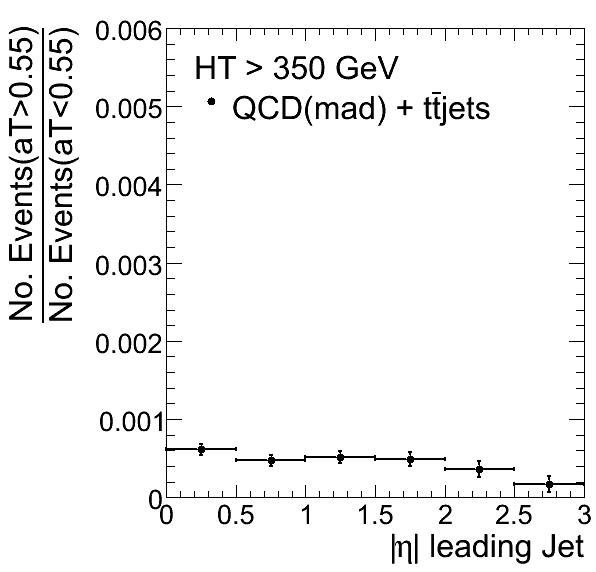
\includegraphics[scale=0.38]{./plots/RaT-TTbarVsQCD.png}} 
\end{minipage}
\begin{minipage}[b]{0.5\linewidth}
\centering
{\label{fig:$H_{T}$}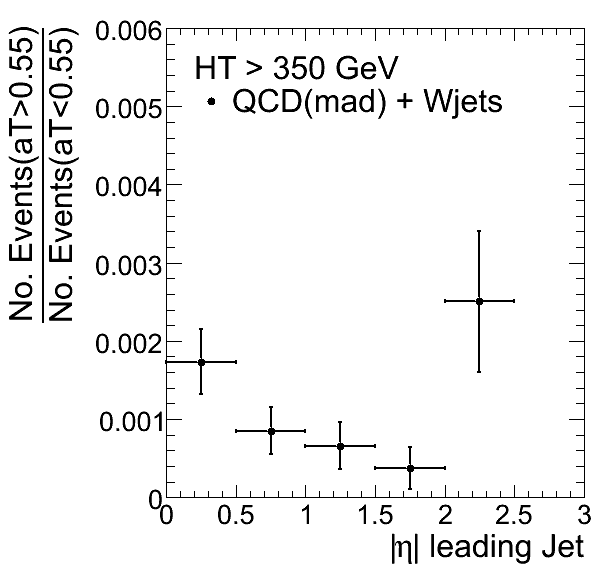
\includegraphics[scale=0.38]{./plots/RaT-WVsQCD.png}} 
\end{minipage}
\caption{\textit{The $R_{\alpha T}$ versus the leading jet $\eta$, for the $t\bar{t} + \textrm{jets}$ (left) and $W + \textrm{jets}$ (rig$H_{T}$), separately.} }
\label{fig:bkgsep}
\end{figure}

%\newpage
\begin{figure}[h!]
%\begin{minipage}[b]{0.5\linewidth} % A minipage that covers half the page
\centering
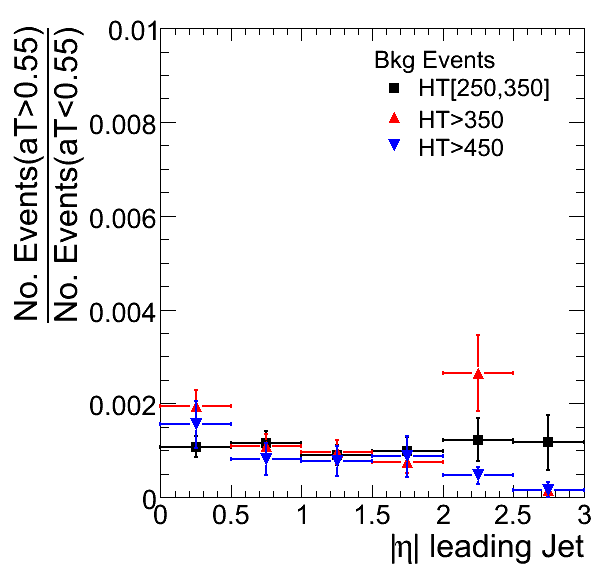
\includegraphics[scale=0.38]{./plots/RaT-Bkg.png}
%\end{minipage}
%\hspace{0.1cm} % To get a little bit of space between the figures
%\begin{minipage}[b]{0.5\linewidth}
%\centering
%\includegraphics[scale=0.38]{}
%\end{minipage}
\caption{\textit{The $R_{\alpha T}$ versus the leading jet $|\eta|$ for the SM background-only hypothesis, in three $H_{T}$ bins [250, 350], [350, inf], [450, inf].} }
\label{fig:id1}
\end{figure}

\begin{figure}[h!]
\begin{minipage}[b]{0.5\linewidth}
\centering
{\label{fig:aT}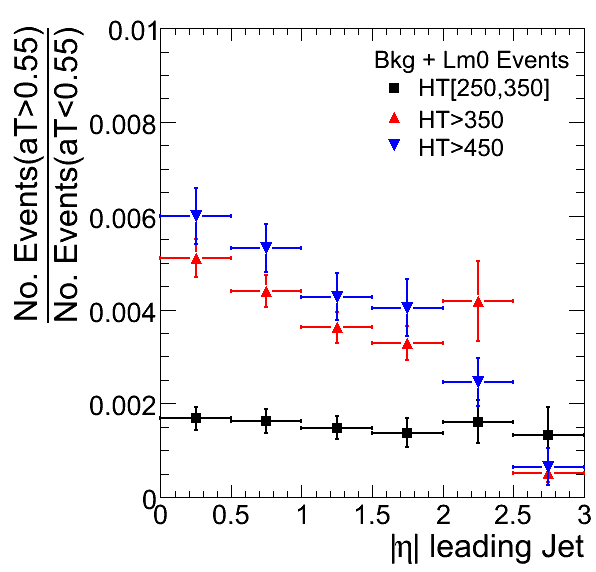
\includegraphics[scale=0.38]{./plots/RaT-LM0.png}} 
\end{minipage}
\begin{minipage}[b]{0.5\linewidth}
\centering
{\label{fig:m$H_{T}$}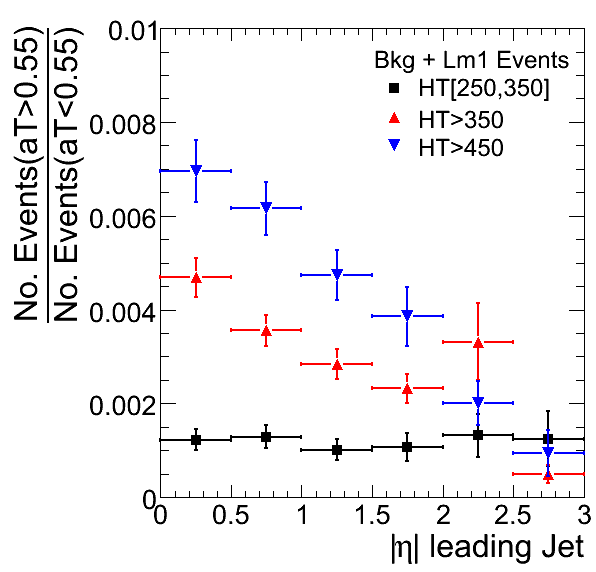
\includegraphics[scale=0.38]{./plots/RaT-LM1.png}} 
\end{minipage}
\caption{\textit{The $R_{\alpha T}$ versus the leading jet $|\eta|$ for the SUSY signal plus SM background hypothesis, in three $H_{T}$ bins [250, 350], [350, inf], [450, inf].} }
\vspace{5mm}
\label{fig:id2}
\end{figure}

\begin{comment}
\begin{figure}[h!]
\begin{minipage}[b]{0.5\linewidth} % A minipage that covers half the page
\centering
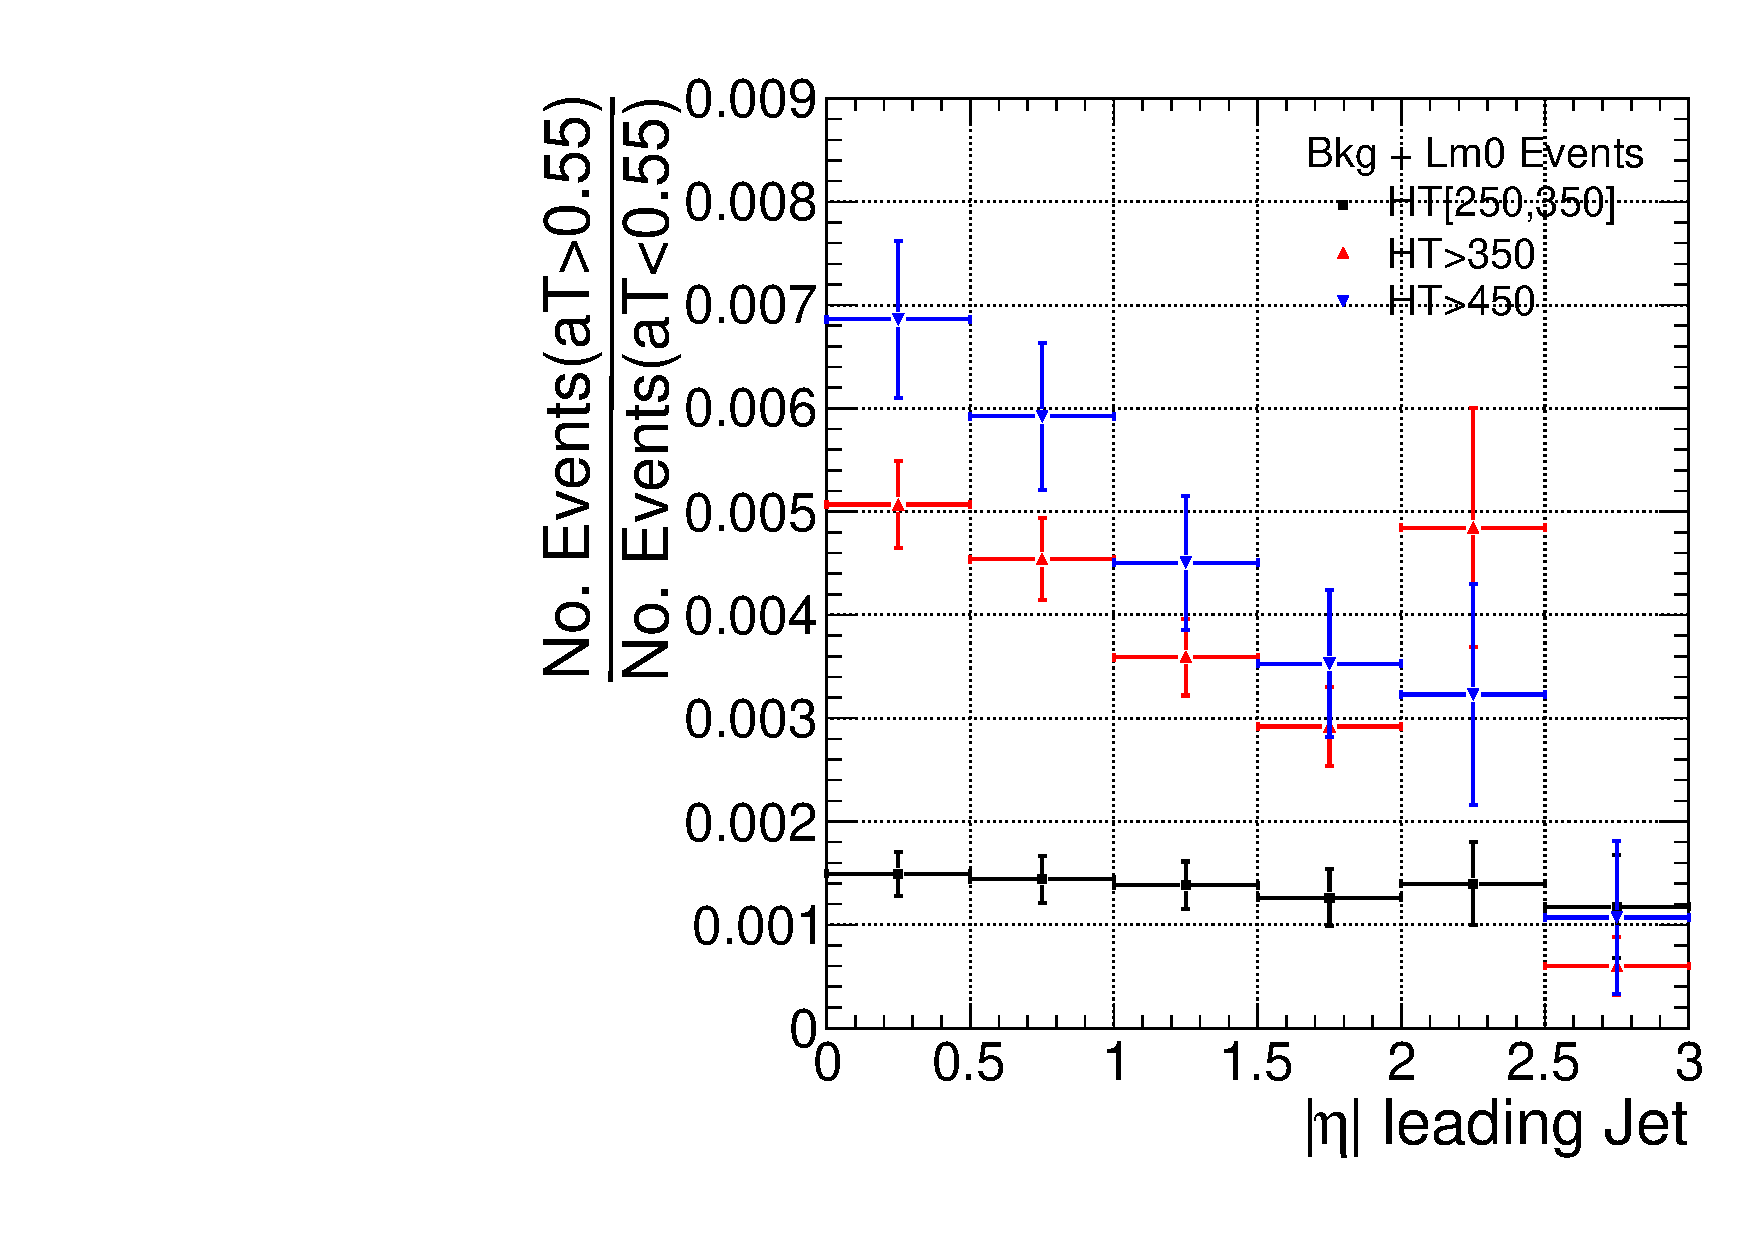
\includegraphics[scale=0.38]{./plots/aT-NT7-Lm0-MCerr}
\end{minipage}
\hspace{0.1cm} % To get a little bit of space between the figures
\begin{minipage}[b]{0.5\linewidth}
\centering
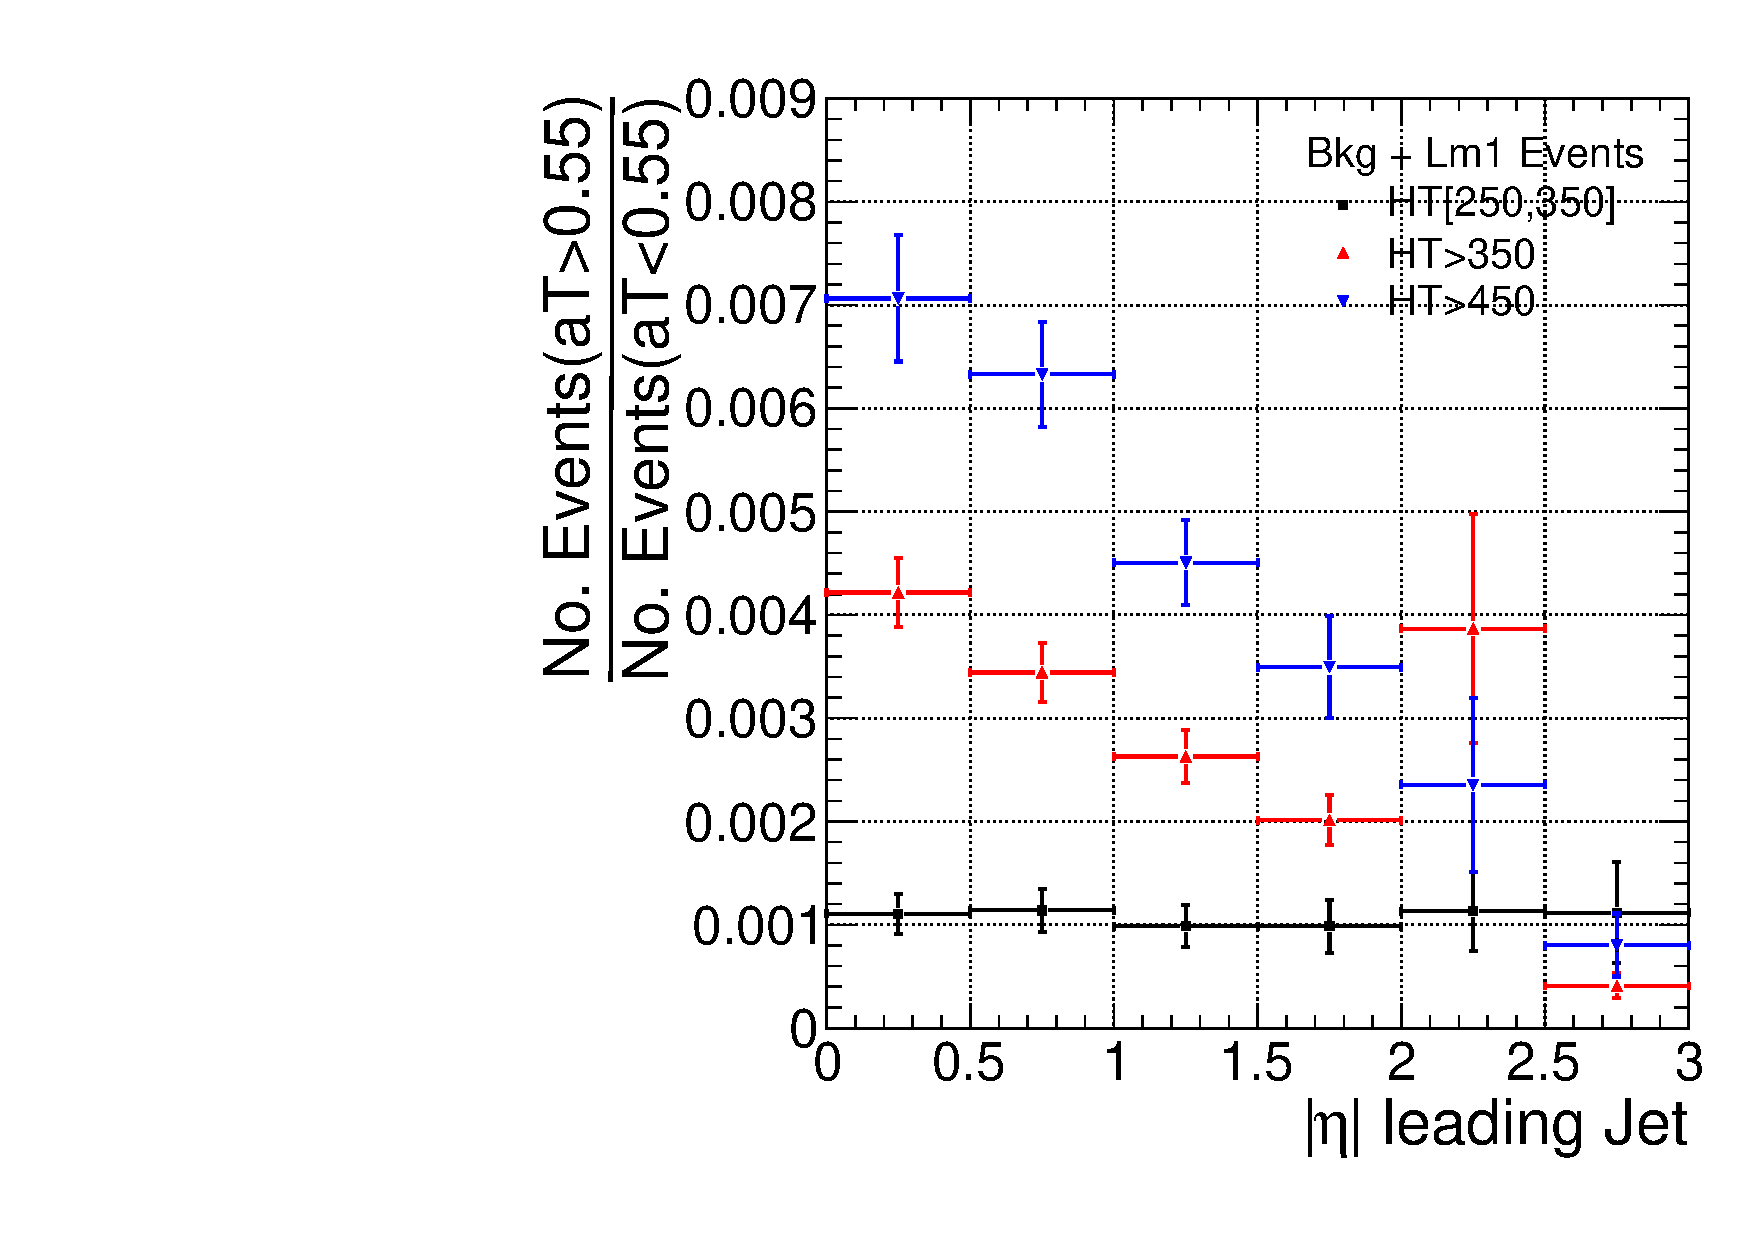
\includegraphics[scale=0.38]{./plots/aT-NT7-Lm1-MCerr}
\end{minipage}
\caption{\textit{The $R_{\alpha T}$ versus the leading jet $\eta$ for the SUSY signal plus SM background hypothesis, in three $H_{T}$ bins [250, 350], [350, inf], [450, inf].} }
\vspace{5mm}
\label{fig:id3}
\end{figure}
\end{comment}

%\clearpage

\subsection{Fitting $R_{\alpha T}$ vs eta}

This section describes an attempt to quantify the procedure of establishing a New Physics deviation from the SM background. A first method is tried by fitting the distributions of RaT vs the $|\eta|$ of the leading jet with a 1st degree polynomial ($p0 + p1 \cdot |\eta|$) using the $\chi^{2}$ method. The parameters of the fit, intercept and slope, for the background-only, as well as the signal-plus-background (background-plus-LM0 and background-plus-LM1) hypotheses have been plotted in bins of $H_{T}$ on figure ~\ref{fig:sum1}. One can easily observe the following:
\begin{enumerate}
 \item The background-only scenario shows flat distributions for both parameters as a function of $H_{T}$, which justifies the assumption of a constant RaT vs $|\eta|$. Instead, the fitting curves for both SUSY scenarios get an increasing incline as the $H_{T}$ threshold rises, leading to a clear distinguish from the background-only case.

\item Two regions in $H_{T}$ can be defined, depending on whether the SUSY signal is either suppressed or pronounced. A very first approach is to select the region with $H_{T}$ threshold below 300 GeV as the ``control region'' and the region $H_{T}>300$~GeV as the ``signal enriched'' region. By this technique and taking into account the flatness of the background distribution, we gain the advantage of estimating the background contribution directly from the data without using any MC-driven methods. We estimate the contribution from the control region and then extrapolate to higher $H_{T}$ regions. This leads inevitably to an over-estimation of the background, which still itself gives a ``safety factor'' which is important when dealing with early data.
\end{enumerate}

\begin{figure}[h!]
\begin{minipage}[b]{0.5\linewidth}
\centering
{\label{fig:m$H_{T}$ov$H_{T}$}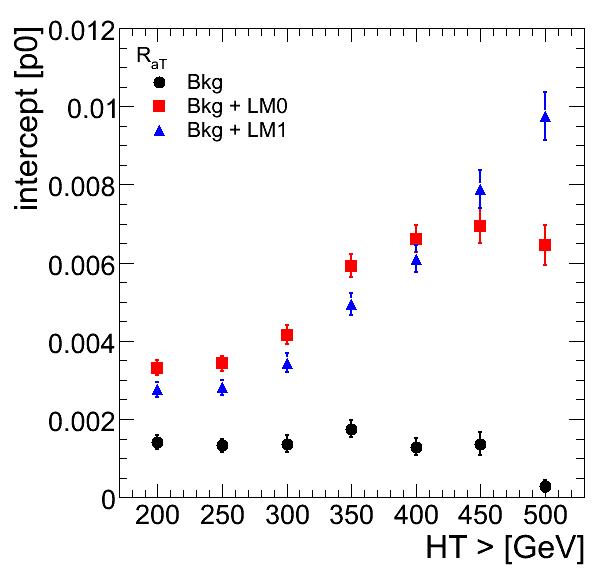
\includegraphics[scale=0.38]{./plots/aT-p0.png}} 
\end{minipage}
\begin{minipage}[b]{0.5\linewidth}
\centering
{\label{fig:$H_{T}$}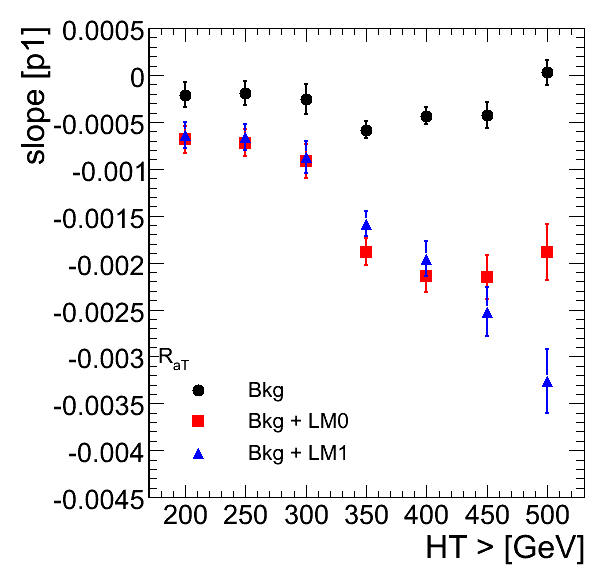
\includegraphics[scale=0.38]{./plots/aT-p1.png}} 
\end{minipage}
\caption{\textit{The fit to the $R_{\alpha T}$ vs $|\eta|$ curves, with a one-degree polynomial $f(|\eta|)= p0 + p1 \cdot |\eta|$, in bins of the $H_{T}$. Left figure shows the intercept ($p0$) values, and rig$H_{T}$ figure shows the slope ($p1$) values, in each $H_{T}$ bin, as extracted from the fit. Error bars assigned use the full MC statistics.  } }
\label{fig:sum1}
\end{figure}

\begin{figure}[h!]
\vspace{5mm}
\begin{minipage}[b]{0.5\linewidth}
\centering
{\label{fig:m$H_{T}$ov$H_{T}$}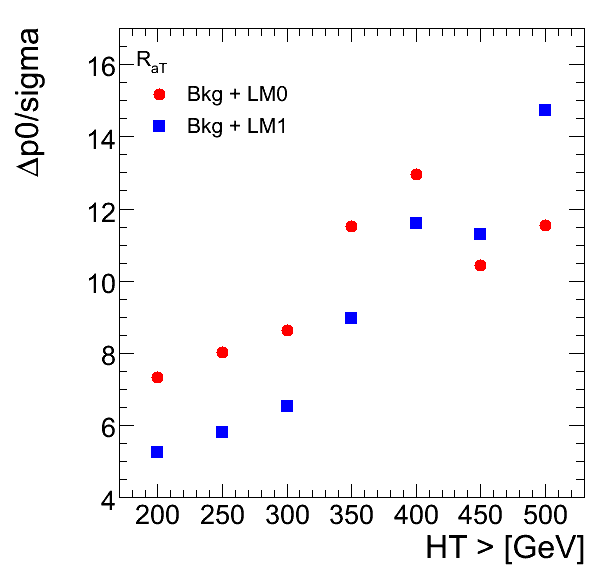
\includegraphics[scale=0.38]{./plots/aT-Dp0OvSigma.png}} 
\end{minipage}
\begin{minipage}[b]{0.5\linewidth}
\centering
{\label{fig:$H_{T}$}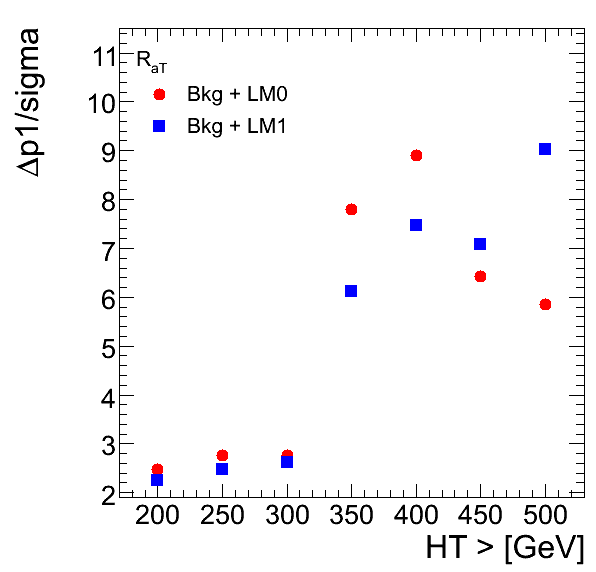
\includegraphics[scale=0.38]{./plots/aT-Dp1OvSigma.png}} 
\end{minipage}
\caption{\textit{A measure of the ``significance'' for establishing a SUSY deviation to the SM expectations: i) $\Delta p0 = p0_{fit}^{tot} - p0_{fit}^{bkg}$ - left figure - and $\Delta p1 = p1_{fit}^{tot} - p1_{fit}^{bkg}$ - rig$H_{T}$ figure -, divided by $\sigma = \sqrt{\sigma_{tot}^{2} + \sigma_{bkg}^{2}}$, in bins of $H_{T}$.  }}
\label{fig:sum2}
\end{figure}

Moving one step forward, we try to estimate the significance of the difference between the measured parameters (p0 and p1) with the presence of signal and the expected values in the background-only case. Thus, we calculate the quantity $\Delta p_{i} / sigma$, where:
\begin{eqnarray}
\Delta p_{i} = p_{i, fit}^{tot} - p_{i_fit}^{bkg},  \\
\sigma =  \sqrt{ (\delta (p_{i, fit}^{tot}))^{2} + (\delta (p_{i, fit}^{bkg}))^{2} } 
\end{eqnarray}
with the index $i$ corresponding to the two parameters of the fitting function.
<<<<<<< deviation.tex
In figure 13 (a) and (b), we plot this quantity for different HT bins, for the parameters p0 and p1 respectively, testing the bkg+LM0 and bkg+LM1 scenarios. When dealing with real data, the parameter values and the corresponding errors for the background-only case will be taken directly from the ``control region''. The difference in the intercept between the signal-plus-background and background-only cases, is more than 5 sigma in the low HT regions, and gets bigger, as expected, for higher HT thresholds. The difference in the slope though, becomes more important (above 5 sigma) for HT values above 350 GeV. This reinforces the assumption of selecting the region with $H_{T}<300$~GeV as a ``control region''.

\subsection{Alternatives variables to HT}
HT was chosen for this method as SM processes dominate in the low region, and potential SUSY signal in the higher region. Another typical observables that exhibits this behaviour is the effective mass, $M_{eff}$, for which the distribution is shown in Figure . We repeat the previous analysis, using regions of $M_{eff}$ instead of H$_{T}$, for comparison, whilst having imposed a 350GeV cut on H$_{T}$.The plota in figure show the same deviation from background hypothesis as was seen for HT. The deviation is in this case more rapid though it is clearly dependent on the choice of Meff bins. Using the 


=======
In figure \ref{tab:sum2}, we plot this quantity for different $H_{T}$ bins, for the parameters p0 (left) and p1 (right) respectively, testing the background-plus-LM0 and background-plus-LM1 scenarios. When dealing with real data, the parameter values and the corresponding errors for the background-only case will be taken directly from the ``control region''. The difference in the intercept between the signal-plus-background and background-only cases, is more than 5 sigma in the low $H_{T}$ regions, and gets bigger, as expected, for higher $H_{T}$ thresholds. The difference in the slope though, becomes more important (above 5 sigma) for $H_{T}$ values above 350 GeV. This reinforces the assumption of selecting the region with $H_{T}<300$~GeV as a ``control region''.>>>>>>> 1.8
